\chapter{METHODOLOGY}

\section{Introduction}

This chapter presents a comprehensive and mathematically rigorous exposition of the engineering
methodology developed to realize the multi-objective autonomous navigation architecture established
in Chapter 1. The algorithmic and validation frameworks designed herein are systematically
structured around three core pipeline milestones: first, the mathematical formulation of a
two-and-a-half-dimensional (2.5D) A* graph-search algorithm that directly embeds physical
three-dimensional step distances (3DSD), localized slope magnitudes (SM), and an adjustable slope
weight parameter ($\lambda$) into a unified multi-terrain cost function; second, the development of
a post-processing B-spline trajectory refinement module that couples continuous curve optimization
with a high-frequency discrete sampling check to actively enforce vehicle climbability thresholds
and boundary constraints; and third, the implementation of a simulation-based benchmarking suite to
evaluate the terrain-aware pathfinder directly against a conventional flat 2D baseline planner.
Consequently, this introductory framework serves as the structural foundation for the algorithmic
mechanics, kinematic verifications, and empirical data trends detailed throughout this study.

To ensure strict reproducibility and technical transparency within a simulated field environment,
this chapter details the explicit computational components, procedural pipelines, and analytical
strategies used to validate the system. It describes the synthesized digital assets, the
computational processing infrastructure, the step-by-step terrain grid synthesis, the parameter
configuration matrices, and the data acquisition protocols. Each architectural choice is
systematically justified relative to the specific technical gaps identified in contemporary field
robotics literature, ensuring that the resulting metrics directly address the study's core research
questions. By executing these sequential validation protocols within a highly controlled virtual
sandbox, this methodology establishes a reliable, repeatable, and hardware-scalable environment for
quantifying the exact safety and efficiency gains achieved by the proposed terrain-aware framework.

\section{Research Design and Experimental Architecture}

The validation of the proposed motion planning architecture relies on a deterministic,
simulation-based experimental design configured around a comparative performance benchmarking
paradigm. This systemic architecture is engineered to quantitatively evaluate the operational
efficacy of the proposed terrain-aware 2.5D A* algorithm against a conventional flat 2D planar
baseline under rigidly controlled and perfectly reproducible environmental conditions. Developing
this framework within an entirely virtual software sandbox enables the systematic manipulation of
high-dimensional input variables and the precise observation of resulting path characteristics.
Consequently, this digital design choice eliminates the unpredictable logistical overhead, physical
hardware constraints, and safety hazards inherent in physical off-road agricultural field testing,
while guaranteeing absolute mathematical consistency across all evaluation trials.

To thoroughly examine the runtime behavior and optimization limits of the pathfinder, the
experimental variables are structured into a multi-tiered evaluation matrix:

\begin{itemize}
    \item \textbf{Terrain Relief Severity Configurations:} The workspace environment is parameterized into three distinct synthetic, deterministic 3D agricultural terrain maps characterizing low-gradient plains, medium-relief hills, and high-relief escarpments. This geometric variation ensures a comprehensive evaluation of the algorithm's topological robustness and structural adaptability across a realistic spectrum of topographical hazards common to unmanaged agricultural fields.

    \item \textbf{Slope Cost Weight Parameter Sweeps ($\lambda$):} The operational influence of surface steepness during graph node expansion is analyzed by systematically sweeping the adjustable slope weight parameter ($\lambda$) across five discrete values: $\lambda \in \{0.0, \allowbreak 0.25, \allowbreak 0.5, \allowbreak 0.75, \allowbreak 1.0\}$. This parameter distribution enables a precise quantitative assessment of how adjusting the penalty weight of localized inclines shifts the trajectory's geometric path optimality.

    \item \textbf{Start-Goal Coordinate Pairs:} To ensure statistical generalizability and eliminate spatial selection bias, three unique, representative start-to-goal coordinate vectors are defined for each distinct terrain profile map.
\end{itemize}

To maintain internal validity and isolate the performance variations caused by these primary
variables, a rigid suite of constant system parameters is uniformly enforced across all
computational trials:

\begin{itemize}
    \item \textbf{Grid Cell Size Map Resolution:} All structural 2.5D elevation matrices are strictly maintained at a uniform coordinate resolution of $500 \times 500$ cells.

    \item \textbf{Maximum Climbable Slope (MCS) Threshold Limit:} A universal hard safety constraint of $\theta_{MCS} = 20^{\circ}$ (representing an operational vehicle gradient limit of approximately 36\% or 0.36 rad) is enforced as a non-negotiable traversability limit. This value models the steepness threshold beyond which the target agricultural platform becomes susceptible to structural slipping or dynamic rollover, rendering such grid coordinates completely impassable.

    \item \textbf{Vegetation Traversal Penalty (VTP) Value:} A fixed scalar cost penalty is uniformly applied to grid coordinates containing dense canopy distributions, reflecting increased locomotion resistance and crop protection boundaries without making the cells strictly forbidden.
\end{itemize}

For robust performance verification, a total of 15 automated evaluation runs are executed per
terrain profile map. This execution matrix comprises evaluating each of the three unique start-goal
coordinate vectors across the five distinct slope cost weight settings. This systematic experimental
architecture provides the comprehensive empirical datasets necessary to satisfy Objective 3,
establishing a clear, multi-variant foundation for performance verification.

\section{Spatial Data Representations and Environmental Modeling}

The environmental modeling pipeline within this computational architecture relies entirely on
structured synthetic data arrays that represent the topographical and semantic layers of the
agricultural workspace. Because this research is conducted within a virtual development sandbox,
these digitized spatial matrices serve as the primary inputs for the navigation stack. Utilizing
pure software-driven environmental configurations guarantees that all input geometries remain
perfectly controlled, mathematically consistent, and reproducible across all simulation trials.

To construct a high-fidelity workspace for algorithmic evaluation, the environmental datasets are
organized into four interconnected core representations:

\begin{itemize}
    \item \textbf{Simulation-Derived 3D Point Cloud Data (.pcd Format):} The foundational spatial data originates as dense three-dimensional (3D) point clouds stored in the standard .pcd file format, mimicking the raw spatial coordinate vectors output by high-resolution field Light Detection and Ranging (LiDAR) sensor suites. These unorganized geometric matrices provide the high-fidelity structural foundation needed to synthesize varied, repeatable terrain profiles without introducing sensor noise or physical environmental variables.

    \item \textbf{Static 2.5D Elevation Grids:} The raw volumetric .pcd datasets are systematically parsed and converted into structured, static two-and-a-half-dimensional (2.5D) elevation grids. This mapping paradigm correlates horizontal planar coordinates $(x, y)$ with a single, discrete altitude value $z$ for each individual grid cell, striking a highly practical structural balance between the spatial blindness of flat 2D models and the massive computational overhead of full 3D volumetric voxel structures. This heightfield representation remains computationally tractable for real-time edge processing while directly supporting the calculation of localized slope gradients and physical three-dimensional step distances.

    \item \textbf{Single-Layer Vegetation Penalty Mask:} Embedded directly as a semantic cost channel within the baseline 2.5D elevation matrices, this localized matrix flags coordinate regions containing dense crop canopies or wild vegetation. These designated cells are uniformly injected with a fixed cost multiplier ($V_{penalty}$), which alters the node expansion priority during graph search by discouraging vehicle translation through dense vegetation zones to protect crop yield and minimize wheel slip.

    \item \textbf{Synthetic Deterministic 3D Agricultural Terrain Profiles:} The operational workspace is explicitly rendered into three distinct digital terrain models classified by relief severity: low-gradient plains, medium-relief rolling hills, and high-relief escarpments. These synthetic agricultural profiles allow for targeted, isolated stress-testing of the pathfinder across a systematically varied spectrum of topographical complexities, reflecting the realistic geometric hazards encountered by heavy machinery in unmanaged fields.
\end{itemize}

\section{Computational Infrastructure and Software Ecosystem}

The computational validation environment configured for this research comprises a unified software
development stack deployed on dedicated processing hardware. Because this methodology bypasses
physical mechanical instrumentation, the selected software assets and computing hardware serve as
the core infrastructure necessary to compile the navigation logic, execute high-frequency constraint
checks, and render dense geometric terrain environments. Standardizing this digital pipeline ensures
absolute algorithmic repeatability and eliminates external hardware-induced latency fluctuations
across all benchmarking trials.

To manage the processing demands of the multi-objective trajectory simulation, the computational
architecture is partitioned into three primary operational tiers:

\begin{itemize}
    \item \textbf{Hardware Processing Infrastructure:} Computational experiments are executed on a dedicated local processing station. This hardware environment provides the multi-threaded throughput and memory bandwidth required to run dense graph-search operations, spatial heightfield conversions, and continuous B-spline matrix solvers without data throttling.

    \item \textbf{Core Software Environment and Specialized Libraries:} The software architecture is developed within a native Linux/Ubuntu ecosystem using Python as the primary programming language for all algorithmic implementations, spatial simulations, and terminal data parsing. Python is chosen due to its extensive scientific computing ecosystem and robust interpreter performance during rapid prototyping cycles. Within this environment, localized array manipulations and mathematical operations are accelerated using several domain-specific libraries:
    \begin{itemize}
        \item \textbf{NumPy:} Deployed to execute high-performance vectorized cell matrix manipulations, coordinate translations, and fundamental Euclidean distance equations.
        \item \textbf{SciPy:} Utilized for advanced mathematical computing pipelines, specifically managing multi-dimensional spatial filtering during terrain synthesis and solving B-spline knot vectors during path refinement.
        \item \textbf{Matplotlib:} Integrated to visualize data structures by rendering interactive 2.5D heightmaps, comparative trajectory curves, and analytical performance histograms.
    \end{itemize}

    \item \textbf{Downstream Framework Compatibility:} All mapping outputs, cost-map transformations, and pathfinding logic are structurally engineered to adhere to data types compatible with the Robot Operating System 2 (ROS2) and Autoware architectures. This design choice ensures that the developed software modules can transition into production-level autonomy stacks for hardware-in-the-loop (HIL) testing or integration into complex autonomous vehicle ecosystems.
\end{itemize}

\subsection{Reference Physical Platform}

\begin{figure}[htbp]
\centering
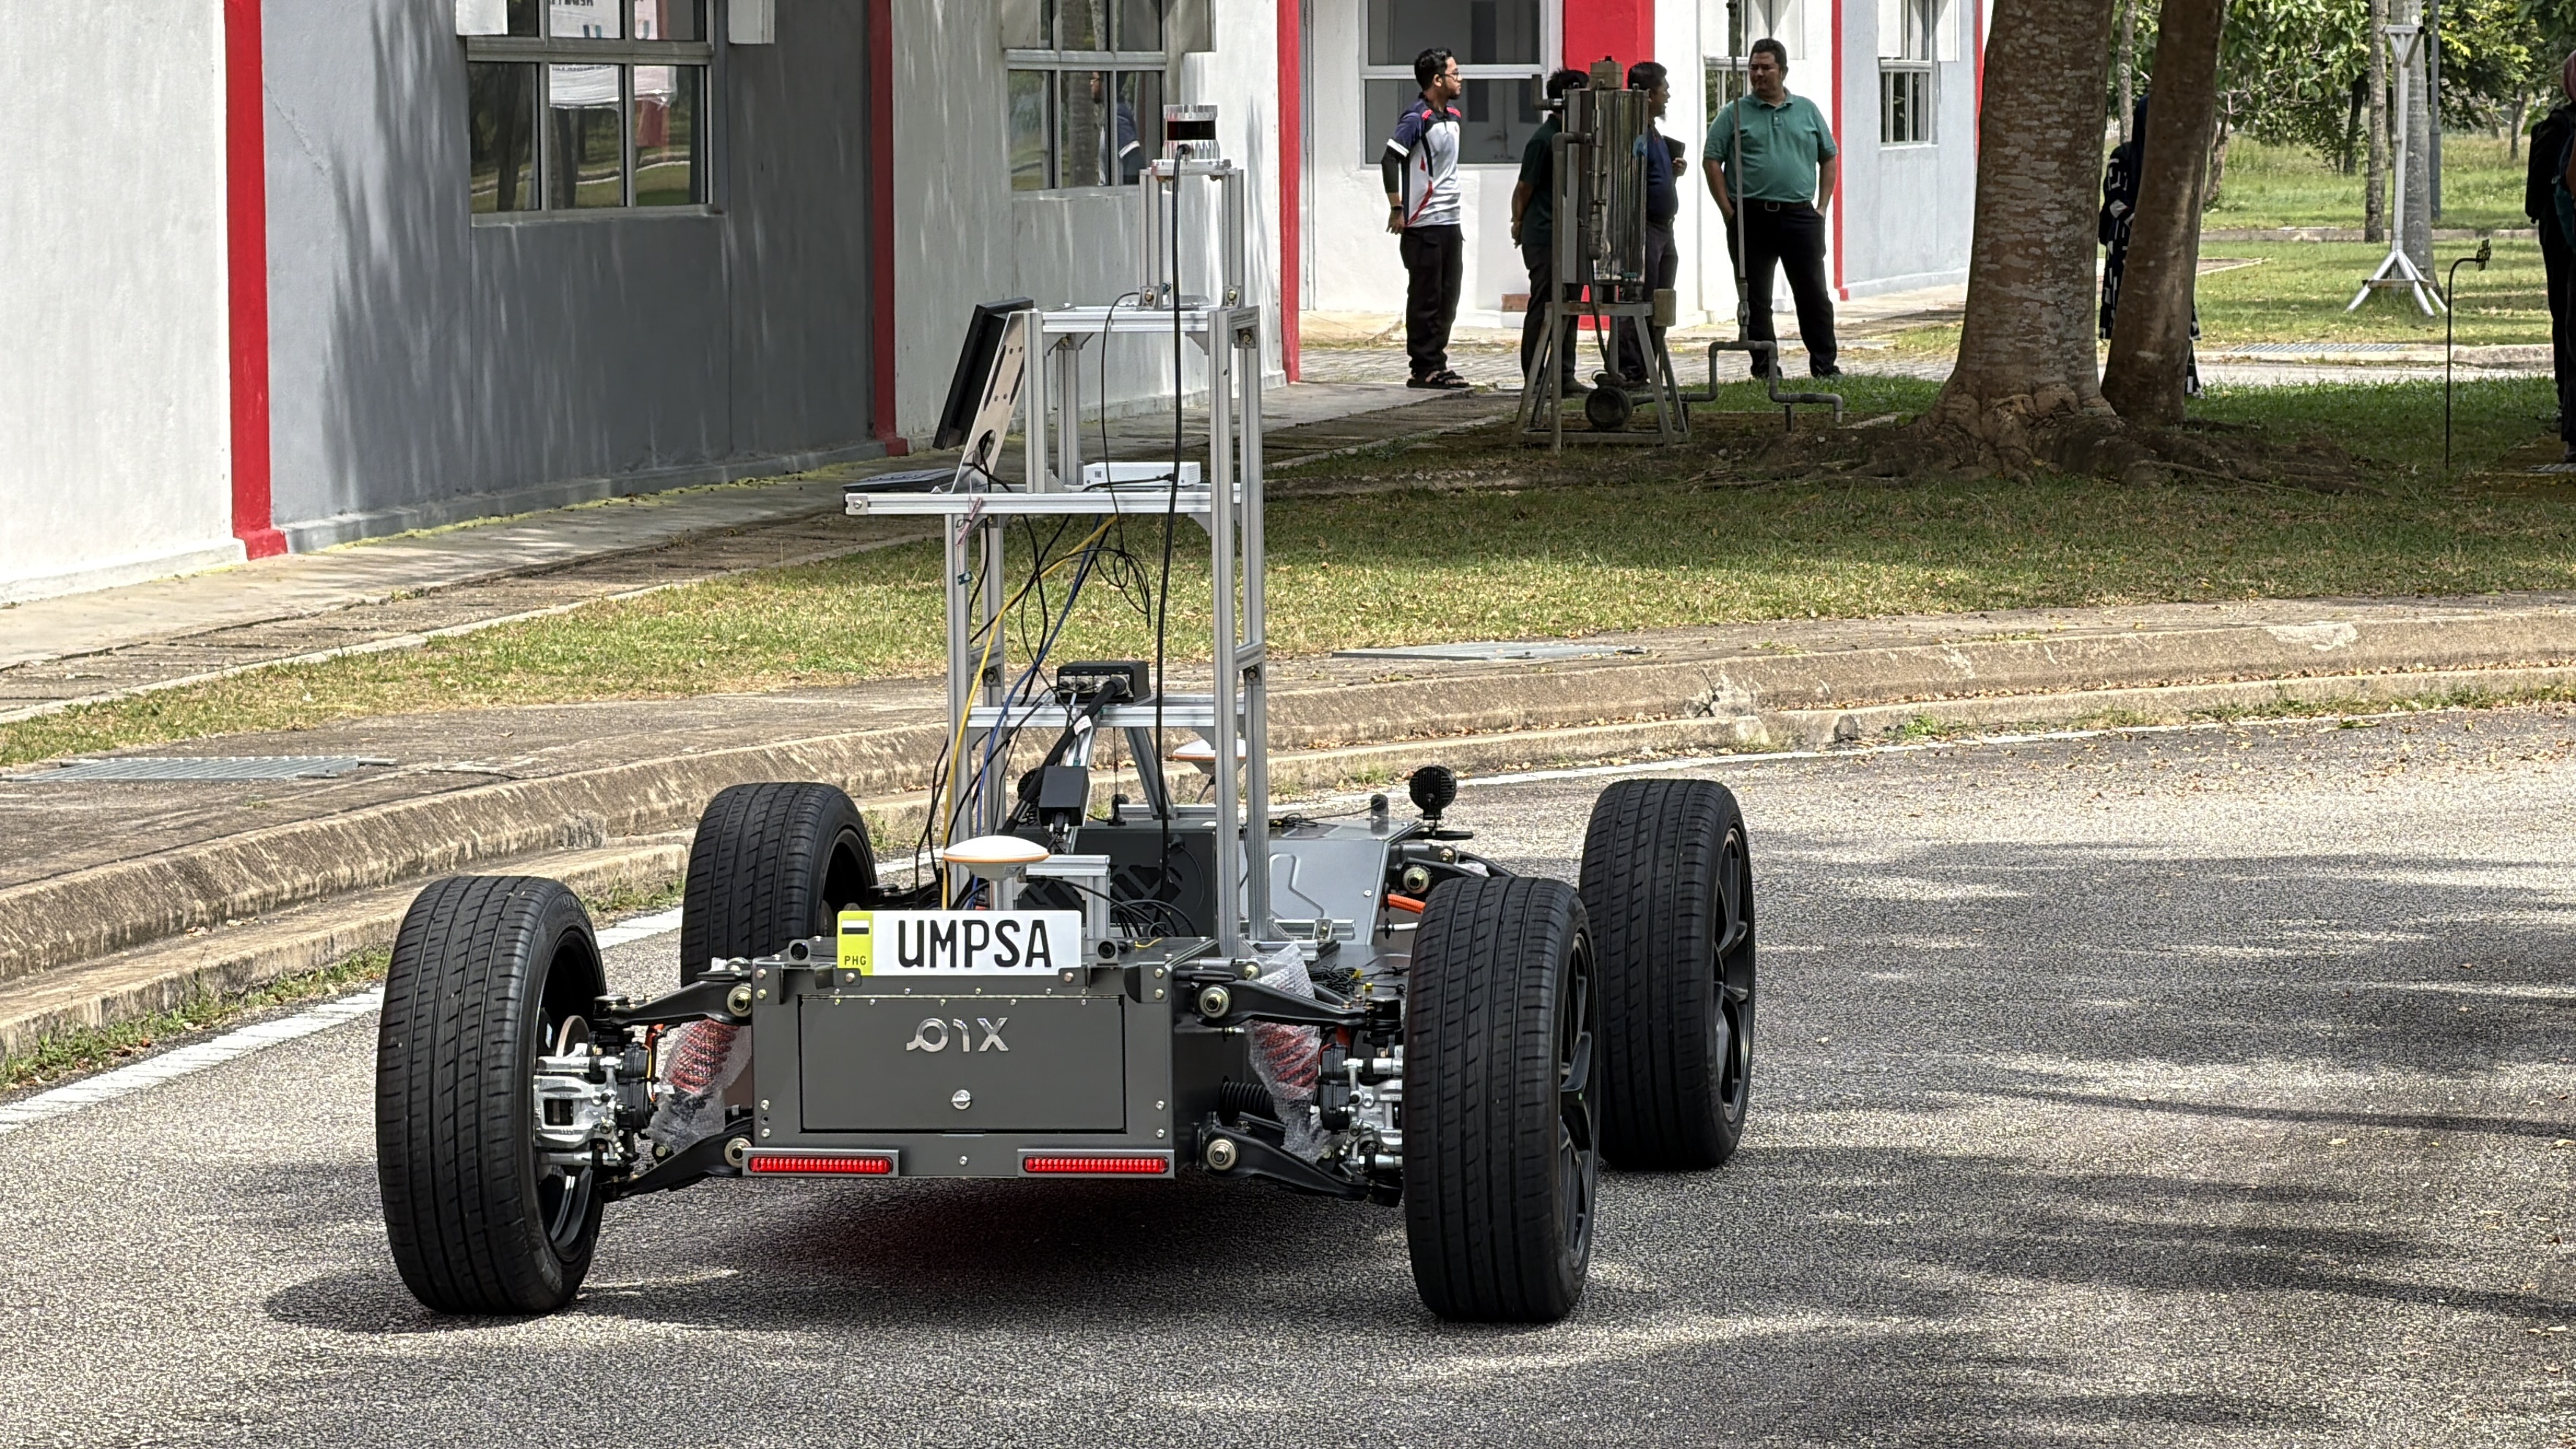
\includegraphics[width=0.95\linewidth]{figures/pixplatform.JPG}
\caption{Autonomous platform used as the target deployment system.}
\label{fig:real_platform}
\end{figure}

To ground the virtual workspace boundaries within realistic operational limits, the kinematic
specifications of the Pix Kit autonomous field platform are integrated as design constraints during
software development. While no physical vehicle trials are conducted within the scope of this
thesis, the platform's real-world parameters---specifically its wheelbase geometry, track width,
center of mass elevation, and electrical powertrain limits---are used to establish the hard Maximum
Climbable Slope ($\theta_{MCS}$) limits enforced within the cost function. Aligning the simulation
parameters with a commercial-grade autonomous chassis ensures that the generated global trajectories
remain safe, practical, and highly relevant for future physical agricultural deployments.

\section{Algorithmic Pipeline and Implementation Procedures}

\begin{figure*}[htbp]
\centering
\resizebox{\textwidth}{!}{%
\begin{tikzpicture}[
    node distance=0.9cm and 0.6cm,
    box/.style={rectangle, draw, rounded corners=2pt, align=center, minimum height=0.9cm, minimum
width=0.78\linewidth, text width=0.74\linewidth, inner sep=4pt, fill=gray!8},
    hbox/.style={rectangle, draw, rounded corners=2pt, align=center, minimum height=0.9cm, minimum
width=0.38\linewidth, text width=0.34\linewidth, inner sep=4pt, fill=gray!8},
    arr/.style={-{Latex[length=1.7mm]}, thick},
    small/.style={font=\scriptsize}
]
    \node[draw, rounded corners=3pt, minimum width=0.82\linewidth, minimum height=2.7cm,
fill=green!5] (scene) {};

    \begin{scope}[shift={(scene.center)}, x=0.82cm, y=0.82cm]
        \coordinate (terrainStart) at (-3.9,-0.55);
        \coordinate (terrainA) at (-2.7,-0.08);
        \coordinate (terrainB) at (-1.6,-0.62);
        \coordinate (terrainC) at (-0.35,0.32);
        \coordinate (terrainD) at (0.95,-0.25);
        \coordinate (terrainE) at (2.3,0.12);
        \coordinate (terrainF) at (3.8,-0.05);

        \fill[green!18] (terrainStart) -- (terrainA) -- (terrainB) -- (terrainC) -- (terrainD) --
(terrainE) -- (terrainF) -- (3.8,-1.15) -- (-3.9,-1.15) -- cycle;
        \draw[thick] (terrainStart) -- (terrainA) -- (terrainB) -- (terrainC) -- (terrainD) --
(terrainE) -- (terrainF);

        \fill[green!45!black] (-2.25,0.02) circle (0.14);
        \fill[green!45!black] (-2.25,0.24) circle (0.1);
        \fill[green!45!black] (-2.43,0.1) circle (0.1);
        \fill[green!45!black] (-2.07,0.1) circle (0.1);
        \fill[green!45!black] (2.45,0.04) circle (0.14);
        \fill[green!45!black] (2.45,0.26) circle (0.1);
        \fill[green!45!black] (2.27,0.12) circle (0.1);
        \fill[green!45!black] (2.63,0.12) circle (0.1);

        \draw[orange!80!black, line width=1.2pt] (-3.35,-0.18) .. controls (-2.2,0.55) and
(-1.1,-0.85) .. (0.05,-0.02) .. controls (1.1,0.72) and (2.0,-0.18) .. (3.2,0.05);
        \draw[blue!70!black, dashed, line width=1pt] (-3.35,-0.32) .. controls (-2.3,0.02) and
(-1.05,-0.28) .. (0.02,-0.12) .. controls (1.08,0.08) and (2.0,-0.02) .. (3.2,-0.02);

        \draw[fill=gray!25] (-0.75,-0.12) circle (0.14);
        \draw[fill=gray!25] (-0.25,0.06) circle (0.14);
        \draw[fill=gray!35, rounded corners=1pt] (-0.95,0.02) rectangle (-0.02,0.44);
        \draw[thick] (-0.7,0.44) -- (-0.7,0.7);
        \draw[thick] (-0.28,0.44) -- (-0.28,0.7);
        \draw[thick] (-0.86,0.28) -- (-1.08,0.42);
        \draw[thick] (-0.12,0.28) -- (0.1,0.42);
        \fill[black] (-0.74,0.24) circle (0.02);
        \fill[black] (-0.26,0.24) circle (0.02);

        \node[small, align=center] at (-0.48,1.02) {Ground robot on uneven terrain};
        \node[small, align=center] at (2.7,0.82) {Vegetation region};
        \node[small, text=orange!80!black] at (2.3,-0.68) {raw path};
        \node[small, text=blue!70!black] at (0.95,-0.92) {smoothed path};
    \end{scope}

    \node[box, below=of scene] (pcd) {Point-cloud map input in .pcd format (e.g., Autoware or ROS2
mapping output)};
    \node[hbox, below left=0.9cm and 0.2cm of pcd] (ros2) {Conventional ROS2 planning branch: 2D
occupancy-grid map and planar A*};
    \node[hbox, below right=0.9cm and 0.2cm of pcd] (grid) {Proposed branch: rasterization into a
2.5D elevation grid with vegetation layer};
    \node[hbox, below=of ros2] (ros2out) {Resulting baseline: computationally efficient route with
limited terrain awareness};
    \node[hbox, below=of grid] (astar) {A* search with slope-feasibility filtering and terrain-aware
traversal cost};
    \node[hbox, below=of astar] (smooth) {B-spline refinement followed by sampled boundary,
vegetation, and slope validation};
    \node[hbox, below=of smooth] (metrics) {Evaluation of path length, energy proxy, travel-time
proxy, runtime, and turn-angle reduction};

    \coordinate (split) at ([yshift=-0.35cm]pcd.south);
    \draw[arr] (scene.south) -- (pcd.north);
    \draw[arr] (pcd.south) -- (split);
    \fill (split) circle (1.1pt);
    \draw[arr] (split) -| node[pos=0.58, above, fill=white, inner sep=1pt] {\scriptsize 2D method}
(ros2.north);
    \draw[arr] (split) -| node[pos=0.58, above, fill=white, inner sep=1pt] {\scriptsize 2.5D method}
(grid.north);
    \draw[arr] (ros2.south) -- (ros2out.north);
    \draw[arr] (grid.south) -- (astar.north);
    \draw[arr] (astar.south) -- (smooth.north);
    \draw[arr] (smooth.south) -- (metrics.north);
\end{tikzpicture}
}
\caption{Planning overview with a terrain-scene diagram, followed by point-cloud map input in .pcd format (as commonly produced in Autoware/ROS2), and a split comparison between conventional 2D planning and the proposed 2.5D terrain-aware branch.}
\label{fig:planning_pipeline}
\end{figure*}

\subsection{Point Cloud Rasterization and 2.5D Grid Generation}

The initial phase of the methodology establishes the foundational environmental workspace by
transforming unstructured, high-density three-dimensional (3D) spatial coordinate vectors into a
discretized topology optimized for graph-search operations. This data transformation process
operates through three tightly coupled execution steps:

\begin{itemize}
    \item \textbf{Volumetric Data Input:} The pipeline initializes by loading synthetic 3D point cloud datasets (.pcd format) characterizing the three benchmark agricultural terrain profiles (low-gradient plains, medium-relief rolling hills, and high-relief escarpments). These unorganized point matrices provide the true baseline geometric information of the simulated agricultural workspace.

    \item \textbf{Planar Projection and Rasterization:} The raw spatial points are orthogonally projected onto a horizontal coordinate ground plane parameterized by horizontal coordinates $(x, y)$ and discretized into a uniform, static two-and-a-half-dimensional (2.5D) grid array with a fixed dimension resolution of $500 \times 500$ cells. For each individual grid cell boundary, a single, discrete altitude value $z$ is calculated by extracting and mapping the maximum elevation value from the subset of raw point clouds bounded within that cell's physical spatial footprint. This conservative mapping choice acts as a safety-first bounding envelope, ensuring that micro-topographical height variations, surface ridges, and localized obstacle tops are fully captured to mitigate clearance hazards while completely removing the excessive computational overhead of full volumetric voxel grids.

    \item \textbf{Semantic Costume Mask Integration:} Following heightfield generation, a specialized single-layer semantic vegetation penalty mask is structurally superimposed onto the baseline 2.5D elevation grid. This semantic overlay cross-references coordinate indices to isolate cells containing dense crop canopies or unmanaged ground cover, uniformly injecting a fixed scalar cost modifier ($V_{penalty}$) into the cell's properties. By embedding this soft cost boundary directly into the terrain data array, the local pathfinder is mathematically forced to treat dense vegetation as a high-resistance navigation zone during runtime node expansion, protecting crop yields and minimizing platform slip.
\end{itemize}

\begin{figure}[htbp]
\centering
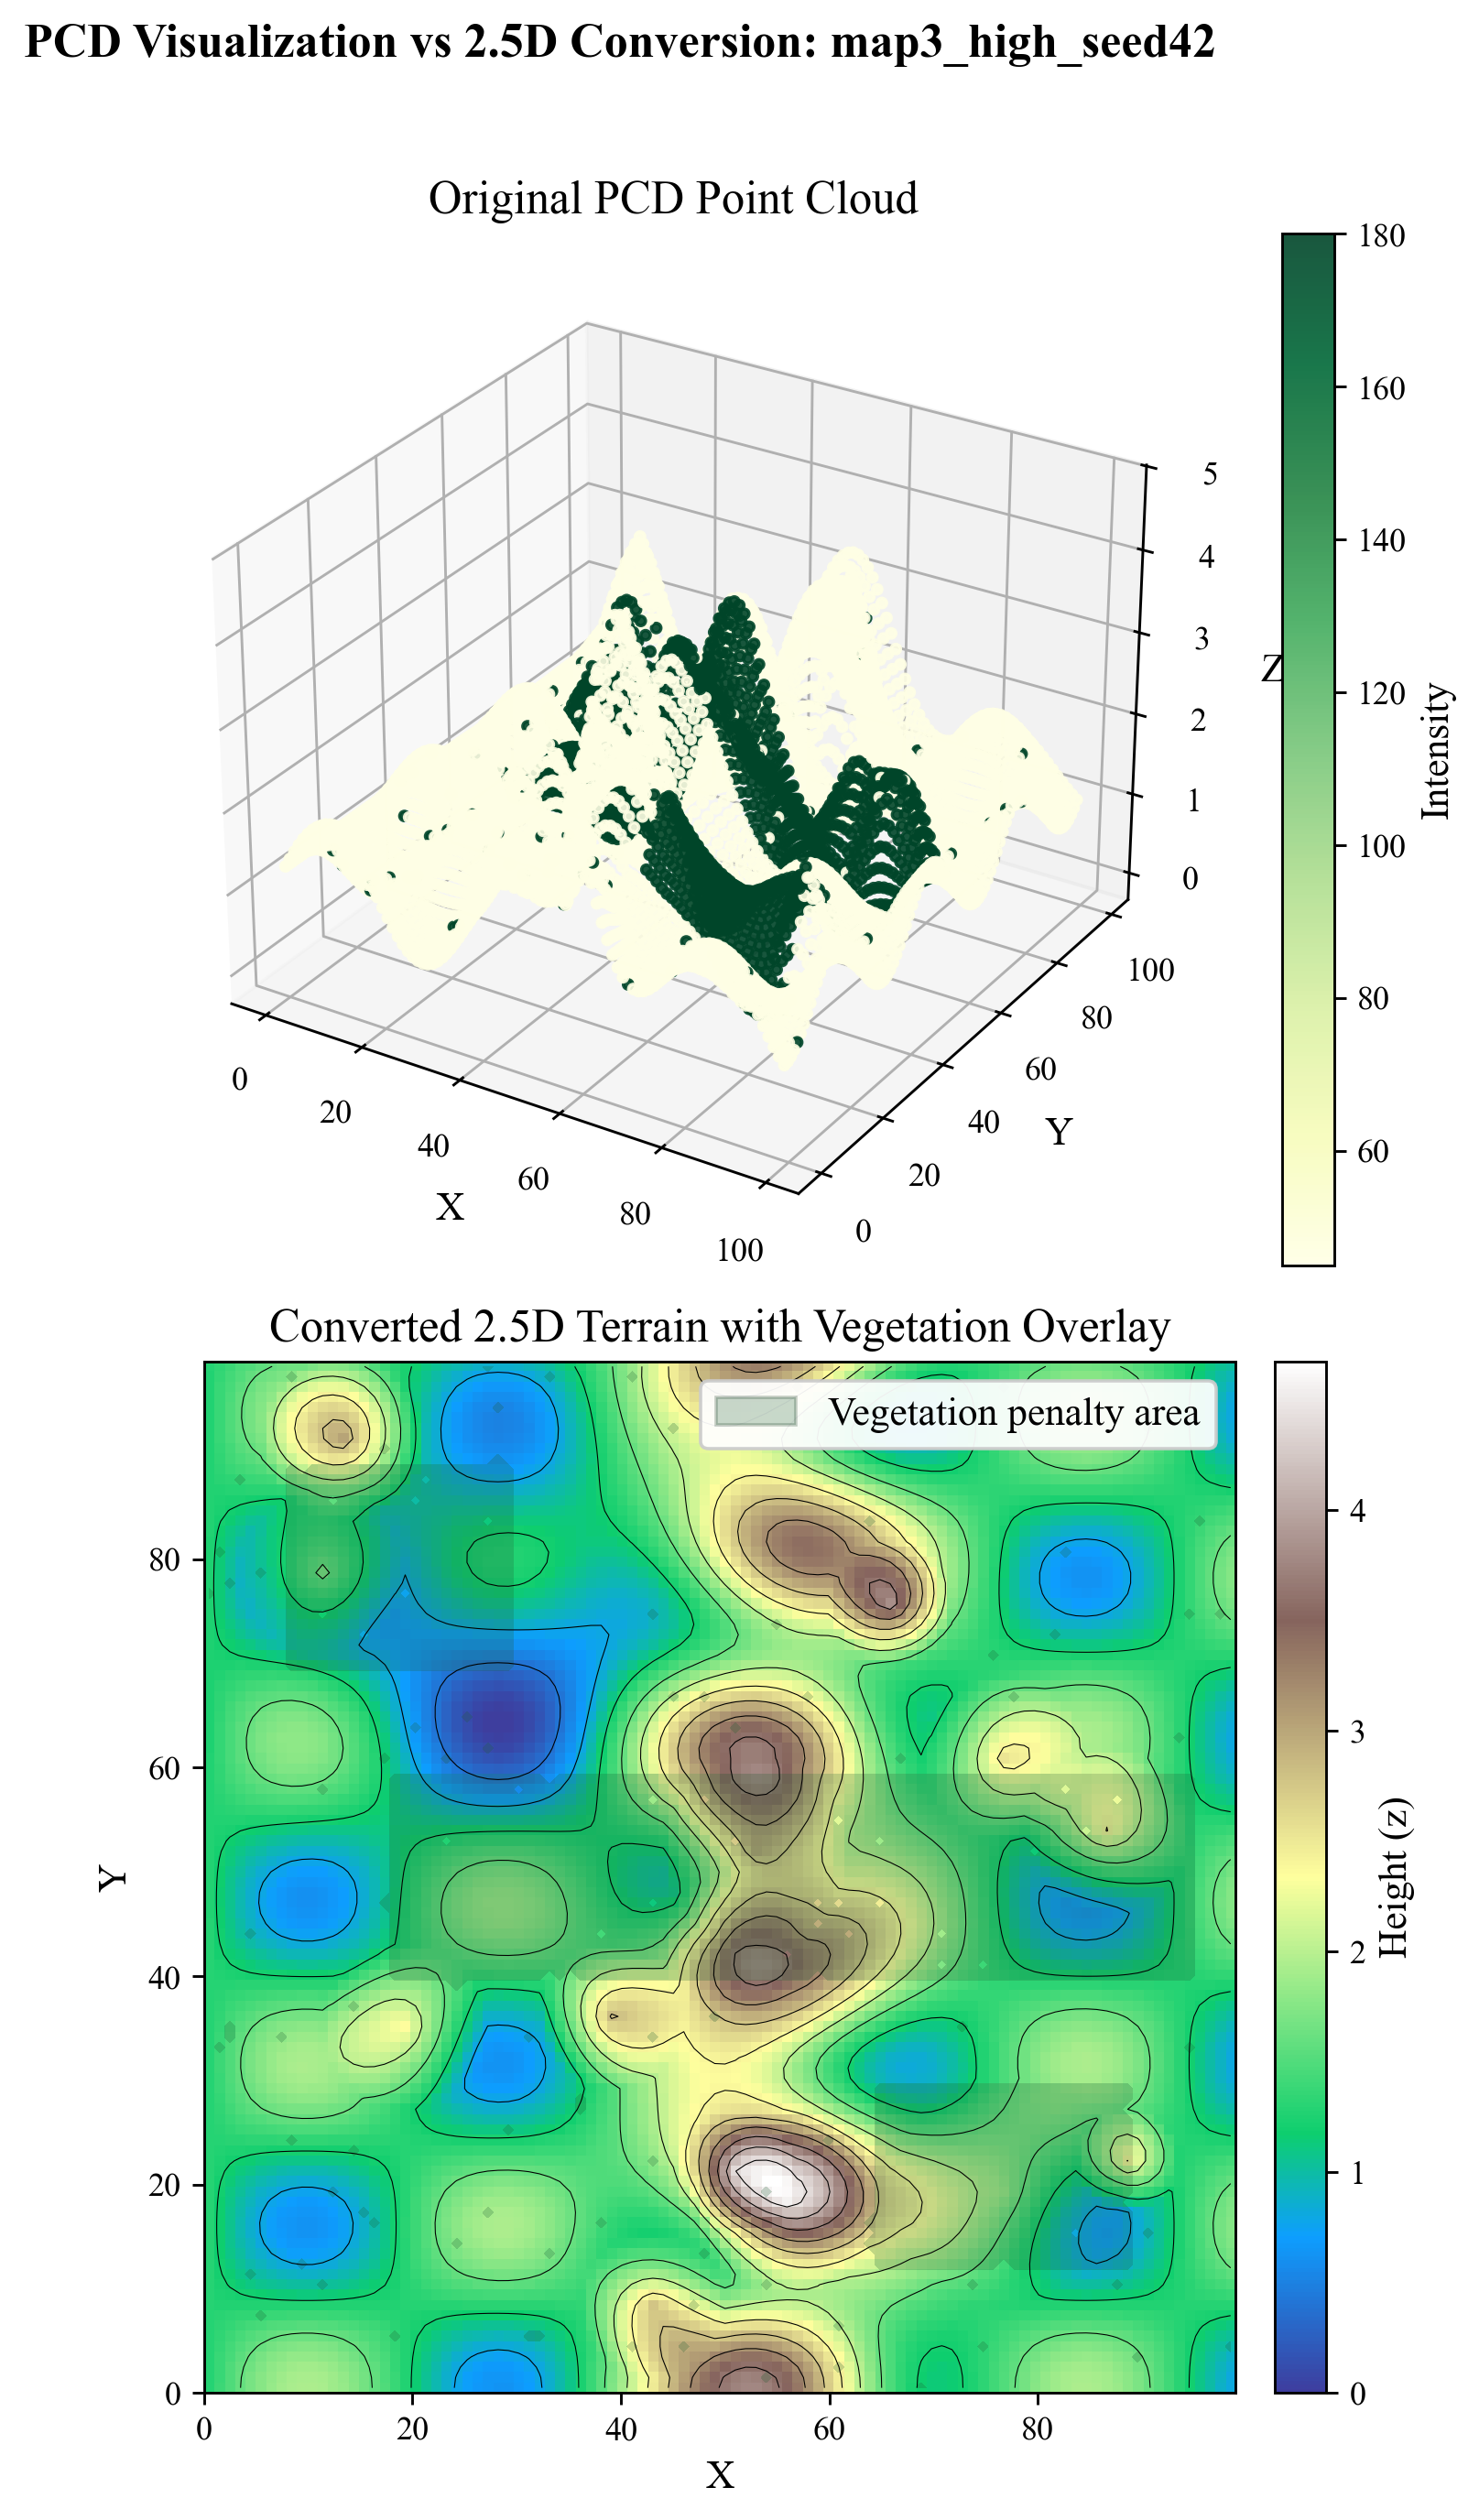
\includegraphics[width=0.95\linewidth, height=0.35\textheight, keepaspectratio]{figures/map3_high_seed42_pcd_vs_25d.png}
\caption{Example preprocessing result. Left: point-cloud visualization of the terrain source. Right: the corresponding 2.5D raster representation used by the planner, including the vegetation penalty region.}
\label{fig:pcd_example_compare}
\end{figure}

\subsection{Formulation of Terrain-Aware Step Traversal Cost (STC)}

To achieve a highly responsive, topology-aware graph expansion under the modified A* path planning
architecture, a novel terrain-aware Step Traversal Cost (STC) function is formulated to evaluate
edge weights between adjacent nodes. This multi-variant cost model directly satisfies the
requirements of Objective 1 by integrating physical three-dimensional step distances ($d_{3D}$),
localized slope magnitudes ($\theta$), a semantic vegetation modifier ($V_{penalty}$), and an
adjustable slope weight parameter ($\lambda$) into a unified optimization metric. For a discrete
translation step from a current parent cell $P$ to an adjacent candidate cell $C$ within an
8-connected neighborhood, the instantaneous traversal cost is modeled via the following structural
equation:

\begin{table}[htbp]
\caption{Nomenclature}
\label{tab:nomenclature}
\centering
\footnotesize
\begin{tabular}{p{0.16\columnwidth} p{0.72\columnwidth}}
\toprule
\textbf{Term} & \textbf{Definition} \\
\midrule
MCS & Maximum climbable slope constraint used to reject infeasible transitions. \\
SCW ($\lambda$) & Slope cost weight controlling the sensitivity of traversal cost to local gradient. \\
VTP ($P_{\mathrm{veg}}$) & Vegetation traversal penalty applied to cells inside the vegetation mask. \\
SM$_{i,j}$ ($\theta$) & Local slope magnitude between neighboring nodes $i$ and $j$. \\
3DSD$_{i,j}$ ($d_{3D}$) & Three-dimensional step distance between nodes $i$ and $j$. \\
STC$_{i,j}$ & Step traversal cost used in the accumulated A* cost. \\
$L_{\mathrm{3D}}$ & Total three-dimensional path length. \\
ECP & Energy consumption proxy. \\
TTP & Travel-time proxy. \\
$I^{\mathrm{veg}}_{i,j}$ & Vegetation indicator for the transition from node $i$ to node $j$. \\
$I^{\uparrow}_{k,k+1}$ & Uphill-motion indicator for path segment $k$ to $k+1$. \\
\bottomrule
\end{tabular}
\end{table}

\begin{equation}
    STC(P, C) = d_{3D}(P, C) + \lambda \cdot \theta(P, C) + V_{penalty}(C)
\end{equation}

\noindent where the constituent geometric and semantic sub-functions are defined and mathematically bounded as follows:

\begin{itemize}
    \item \textbf{Three-Dimensional Step Distance ($d_{3D}$):} This parameter quantifies the true 3D Euclidean distance separating the volumetric geometric centers of parent cell $P$ and candidate cell $C$. Unlike conventional planar planners that rely on 2D horizontal projections---which treat translations over sloped and flat planes identically---the $d_{3D}$ function incorporates heightfield differentials to capture the real physical travel distance and mechanical effort:
    \begin{equation}
        d_{3D}(P, C) = \sqrt{(x_C - x_P)^2 + (y_C - y_P)^2 + (z_C - z_P)^2}
    \end{equation}

    \item \textbf{Local Slope Magnitude ($\theta$):} This metric represents the topographic steepness or spatial gradient established between the center coordinates of cells $P$ and $C$. The slope magnitude is calculated as the arctangent of the ratio of the vertical elevation differential ($\Delta z$) to the horizontal distance ($d_{2D}$) separating the cell centers:
    \begin{equation}
        \theta(P, C) = \arctan\left(\frac{|z_C - z_P|}{d_{2D}(P, C)}\right)
    \end{equation}
    Elevated $\theta$ profiles indicate high-relief terrain features that introduce immediate
kinematic tracking hazards, track slippage, or platform instability.

    \item \textbf{Adjustable Slope Weight Parameter ($\lambda$):} This scalar coefficient scales the mathematical impact of the local slope magnitude on the total accumulative step cost. Swept systematically across five discrete settings within this research design: $\lambda \in \{0.0, \allowbreak 0.25, \allowbreak 0.5, \allowbreak 0.75, \allowbreak 1.0\}$. A higher $\lambda$ value heavily penalizes steep inclines, forcing the graph-search routine to bypass prominent elevation changes in favor of lateral contour paths. This tunability allows field engineers to dynamically realign the navigation system based on vehicle power limits, soil conditions, or operational preferences (e.g., minimizing fuel consumption versus minimizing overall transit distance).

    \item \textbf{Vegetation Traversal Penalty ($V_{penalty}$):} This binary semantic filter evaluates whether candidate cell $C$ falls within the boundaries of the single-layer vegetation mask. If a vegetation hazard is detected, a fixed scalar penalty is added directly to the edge calculation; otherwise, the term is nullified ($V_{penalty} = 0$). This soft constraint influences trajectory selection by guiding the vehicle away from unmanaged crops or dense brush without designating those zones as strictly impassable obstacles.
\end{itemize}

\subsection{Implementation of Modified 2.5D A* Search Algorithm}

The core graph-search architecture underpins a modified A* path planning algorithm configured to
execute across an 8-connected grid network topology. This implementation operates directly on the
compiled elevation matrices, using the previously formulated Step Traversal Cost (STC) to
dynamically alter node cost evaluation. By integrating real-time geometric and semantic terrain
layers into the primary search loop, the pathfinder proactively routes the mobile robot around
untraversable topographical features. The deterministic graph search evaluates and registers
candidate nodes by incorporating these continuous cost metrics into the standard A* heuristic
evaluation framework:

\begin{equation}
    f(n) = g(n) + h(n)
\end{equation}

\noindent where the algorithmic cost components and hard safety filters are integrated as follows:

\begin{itemize}
    \item \textbf{Cost Function Integration ($g(n)$):} The cumulative cost component $g(n)$, which tracks the exact cost accrued from the initial start state to the current node $n$, is calculated by summing the discrete, terrain-aware step traversal costs (STC) incurred during each successive node transition:
    \begin{equation}
        g(n) = \sum_{i=0}^{k} STC(P_i, C_i)
    \end{equation}
    By mapping $g(n)$ directly to the STC function, the algorithm intrinsically considers the
combined effects of the three-dimensional step distance ($d_{3D}$), localized slope magnitude
($\theta$), the user-defined slope weight parameter ($\lambda$), and the semantic vegetation
traversal penalty ($V_{penalty}$) during the live graph exploration phase.

    \item \textbf{Heuristic Function ($h(n)$):} The heuristic function $h(n)$ provides a computationally efficient, goal-directed bias by estimating the remaining traversal cost from the current node $n$ to the terminal goal state. To guarantee mathematical admissibility (ensuring the planner never overestimates the true remaining cost) and secure global optimality, $h(n)$ is parameterized as the true three-dimensional (3D) Euclidean distance between node center coordinates:
    \begin{equation}
        h(n) = \sqrt{(x_{goal} - x_n)^2 + (y_{goal} - y_n)^2 + (z_{goal} - z_n)^2}
    \end{equation}
    This spatial formulation ensures that vertical height field variations between the active search
front and the goal coordinate are accounted for, generating an accurate and admissible heuristic
envelope.

    \item \textbf{Hard Maximum Climbable Slope (MCS) Safety Filter:} To prevent the pathfinder from generating trajectories that violate the hard physical operating limits of the agricultural mobile platform, a proactive safety constraint checker is embedded directly within the neighbor expansion loop. Prior to pushing a valid neighbor node onto the Open List, the local slope magnitude ($\theta$) between parent cell $P$ and candidate cell $C$ is evaluated against the non-negotiable vehicle threshold ($\theta_{MCS}$):
    \begin{equation}
        \text{if } \theta(P, C) > \theta_{MCS} \Rightarrow \text{node } C \text{ is pruned (impassable)}
    \end{equation}
    Any potential step that exceeds this boundary is immediately classified as un-traversable,
forcing the algorithm to treat the target coordinate as a rigid structural obstacle and prune it
from the active search space. This proactive filtering guarantees that all generated raw paths
respect the structural stability limits of the underlying vehicle chassis before entering the
trajectory refinement stage.
\end{itemize}

\subsection{Conventional 2D Baseline Path Planning}

To establish a rigorous mathematical baseline for the comparative analysis executed in Objective 3,
a conventional planar A* algorithm is implemented as a benchmark tracking routine. This control
planner operates exclusively on a flattened, two-dimensional matrix projection of the environment,
completely stripped of continuous vertical height topologies and localized surface gradients. By
executing graph exploration over this simplified configuration layout, the baseline pathfinder
generates standard piece-wise linear trajectories that reflect traditional coordinate routing
methodologies. The planar search routine evaluates grid nodes within a standard 8-connected pixel
neighborhood using the baseline evaluation function:

\begin{equation}
    f_{2D}(n) = g_{2D}(n) + h_{2D}(n)
\end{equation}

\noindent where the internal cost-tracking parameters and obstacle handling mechanisms are formulated as follows:

\begin{itemize}
    \item \textbf{Planar Cost Function ($g_{2D}$):} The cumulative tracking cost $g_{2D}$ is parameterized strictly by the horizontal 2D Euclidean distance separating adjacent cell centers. This formulation completely omits altitude changes ($\Delta z$), treating translations across steep hills and flat plains as energetically and temporally identical:
    \begin{equation}
        g_{2D}(n) = \sum_{i=0}^{k} \sqrt{(x_{C_i} - x_{P_i})^2 + (y_{C_i} - y_{P_i})^2}
    \end{equation}

    \item \textbf{Planar Heuristic Function ($h_{2D}$):} The goal-directed guidance heuristic $h_{2D}$ is similarly constrained to the horizontal coordinate plane, computing the absolute straight-line distance from the active node $n$ to the destination coordinates without factoring in target peak elevations:
    \begin{equation}
        h_{2D}(n) = \sqrt{(x_{goal} - x_n)^2 + (y_{goal} - y_n)^2}
    \end{equation}

    \item \textbf{Binary Obstacle Handling:} To protect the mobile platform from immediate collision failures, macro-topographical features and slope hazards are managed using a strict binary segmentation mask. If a grid cell's maximum elevation profile natively exceeds the vehicle's predefined Maximum Climbable Slope threshold ($\theta_{MCS}$), that coordinate is classified as a hard barrier and pruned from the search envelope. However, unlike the proposed 2.5D A* algorithm, intermediate slope variations, continuous terrain roughness indices, and semantic vegetation costs do not influence the edge weights of passable cells. The baseline planner treats all non-obstacle terrain as a uniform, zero-cost plane, highlighting the technical limitations that lead to tracking lag and mechanical stress when executing planar paths over non-planar agricultural surfaces.
\end{itemize}

\subsection{Open-Uniform B-spline Trajectory Smoothing with Feasibility Checks}

Following the generation of the initial, discrete path waypoints from either the proposed 2.5D A* or
the baseline 2D A* graph-search algorithms, the trajectory is passed into a specialized
post-processing refinement module. This pipeline phase directly satisfies Objective 2 by optimizing
path curvature while actively validating safety and environmental constraints across the continuous
domain. This dual-purpose refinement process operates through two sequential operations:

\begin{itemize}
    \item \textbf{Open-Uniform B-spline Curve Fitting:} The ordered set of discrete waypoints output by the pathfinder is treated as a topological control point matrix to generate an open-uniform B-spline curve. B-spline formulations are chosen for trajectory optimization because of their local support property, which allows for localized geometric adjustments without causing global shape deformation. To achieve smooth, continuous vehicle velocities and bounded lateral acceleration profiles during physical trajectory tracking, the refinement module enforces strict $C^2$ continuity across the parametric curve. Furthermore, using an open-uniform knot vector configuration clamps the terminal endpoints of the spline function, forcing the continuous curve to pass exactly through the original start and goal coordinate coordinates to maintain global boundary alignment.

    \item \textbf{High-Frequency Discrete Sampling Checks:} To ensure that the continuous geometric refinement has not inadvertently shifted trajectory segments onto unsafe terrains, the optimized B-spline curve undergoes a rigorous validation process. The parametric curve equation is evaluated at uniform, high-frequency intervals to generate a dense array of discrete spatial tracking points. At each sampled coordinate along the continuous path, the system executes three synchronized validation routines:
    \begin{itemize}
        \item \textbf{Maximum Slope Threshold Validation:} The instantaneous localized slope derivative of the smoothed trajectory segment is computed and cross-referenced against the vehicle's hard operating limit ($\theta_{MCS}$). If any individual sampled point exhibits a localized incline exceeding this threshold, the entire candidate trajectory is flagged as invalid.
        \item \textbf{Workspace Boundary Compliance:} The spatial coordinates of each sample point are evaluated against the global configuration space dimensions to verify that the continuous path remains fully contained within the authorized operational tracking boundaries of the agricultural terrain map.
        \item \textbf{Vegetation Exposure Verification:} The sample coordinates are mapped directly onto the underlying semantic mask layer to track and limit cumulative vehicle exposure to dense vegetation zones, protecting crop rows from tire damage and preventing wheel slippage.
    \end{itemize}
\end{itemize}

This multi-layered validation routine acts as a strict safety filter during the post-processing
phase, preventing the generation of trajectories that are kinematically smooth but physically
untraversable or unsafe for field operation.

\subsection{Parametric Data Logging}

To ensure an objective and comprehensive benchmarking process, the optimization framework is coupled
with an automated parametric data-logging module. Upon the successful completion and validation of
each trajectory generated by both the proposed 2.5D A* terrain-aware algorithm and the conventional
2D A* baseline planner, the logging system intercepts the workspace state and captures a
high-fidelity quantitative profile. This data package tracks five primary operational metrics: exact
three-dimensional path length ($L_{3D}$), speed-adjusted travel-time proxies (TTP), computational
execution runtimes, uphill-selective energy consumption proxies (ECP), and the adjustable slope
weight coefficient ($\lambda$). These recorded performance vectors are systematically dumped into
structured flat files (.csv format), creating a clean empirical ledger that supports direct
statistical cross-evaluation during the performance verification stage.

\section{Digital Map Synthesis and Environmental Configuration}

The generation of standardized, controlled, and math\-e\-mat\-i\-cal\-ly re\-pro\-duc\-i\-ble
work\-spaces is a necessary pre\-req\-ui\-site for isolating the optimization performance of the
underlying pathfinding routines. Because this research bypasses physical field deployments, the
environmental mapping configurations are generated synthetically to establish clear topographical
benchmarks. This software-driven synthesis process eliminates chaotic real-world variables---such as
dynamic weather conditions, localized GPS multipath interference, or soil shear strength
fluctuations---while ensuring that all input maps share a uniform cell resolution and data layout to
maximize internal validation.

To build out the evaluation workspace, the environmental data synthesis pipeline executes across
four tightly integrated configuration phases:

\begin{itemize}
    \item \textbf{High-Fidelity Point Cloud Generation:} The synthesis begins with programmatically generating dense, three-dimensional (3D) point cloud matrices stored in the standard .pcd file format. These point configurations are mathematically generated to build three distinct agricultural terrain profiles classified by relief severity: low-gradient plains, medium-relief rolling hills, and high-relief escarpments. This geometric step locks in the baseline spatial characteristics for each experimental scenario, ensuring that the primary elevation data remains completely controlled and reproducible across independent testing blocks.

    \item \textbf{Coordinate Rasterization and 2.5D Conversion:} Each synthetic 3D point cloud is parsed through a coordinate projection and rasterization script. This routine compresses the unorganized spatial data points into a static, two-and-a-half-dimensional (2.5D) elevation matrix with a fixed resolution of $500 \times 500$ cells. To maintain absolute safety-first consistency, each individual 2.5D grid coordinate is assigned a single elevation value $z$ derived by extracting the maximum elevation value from the underlying point cloud subset bounded within that cell's spatial footprint, capturing localized surface peaks to mitigate platform clearance hazards.

    \item \textbf{Semantic Vegetation Mask Overlay:} A single-layer semantic penalty mask is programmatically synthesized and overlaid onto the baseline 2.5D heightfields. This matrix matches the global grid dimensions to flag specific coordinates as heavily vegetated zones, such as unmanaged crop rows or dense undergrowth. These designated coordinate blocks are injected with a fixed cost multiplier ($V_{penalty}$), forcing the active search front to treat the vegetation zones as high-resistance paths.

    \item \textbf{Deterministic Start-Goal Vector Definitions:} To prevent spatial selection bias, three unique start-to-goal coordinate vectors are defined for each of the three terrain profile maps. These operational coordinate pairs are chosen to represent varied navigational challenges---such as routing diagonally across steep ridges or skirting extensive vegetation zones---providing a diverse set of test cases. This structured configuration ensures that all digital environmental configurations are uniform in format, controlled in their characteristics, and optimized for automated input into the path planning framework.
\end{itemize}

\section{Verification Framework and Benchmarking Protocols}

The operational performance and structural reliability of the navigation architecture are evaluated
using a deterministic, simulation-based path planning benchmarking suite. Because this research
bypasses physical mechanical deployment, the verification loop relies on software-driven performance
benchmarking to isolate internal system behaviors from external environmental variables. This
rigorous analytical design choice replaces unpredictable laboratory variables with highly
reproducible, software-defined testing boundaries, providing clear, uncompromised empirical evidence
that directly addresses Objective 3.

To systematically map out the operational boundaries and optimization trade-offs of the pathfinder,
the evaluation pipeline is structured into three primary benchmarking domains:

\begin{itemize}
    \item \textbf{High-Fidelity Virtual Environment Testing:} All algorithmic iterations, coordinate expansion loops, constraint checking steps, and structural path visualizations are conducted within a unified virtual simulation sandbox. This fully digitized environment supports precise replication of experiments, isolation of independent design variables, and targeted edge-case testing without the systemic tracking noise, GPS signal degradation, mechanical wear, or structural safety hazards inherent to physical off-road autonomous mobile robot trials.

    \item \textbf{Direct Comparative Benchmarking:} The core verification routine involves a direct comparative analysis between the proposed terrain-aware 2.5D A* pathfinder and the conventional flat 2D A* planar baseline algorithm. By testing both planners over identical coordinate origins under uniform map criteria, this control architecture establishes a clear mathematical contrast. This layout is necessary to isolate and quantitatively demonstrate the precise geometry, runtime, and energy consumption changes gained through multi-dimensional terrain awareness.

    \item \textbf{Systematic Multi-Variant Experimental Matrix:} To gather exhaustive performance profiles and eliminate data anomalies, the benchmarking routine executes across a pre-calculated, automated test grid:
    \begin{itemize}
        \item \textbf{Topographical Testbeds:} The evaluation spans all three synthetic terrain profiles (low-gradient plains, medium-relief rolling hills, and high-relief escarpments), testing the system across varying levels of vertical relief.
        \item \textbf{Boundary Pair Vectors:} Within each individual terrain map, three unique, representative start-to-goal coordinate vectors are used to test a diverse set of obstacle layouts and elevation obstacles.
        \item \textbf{Parametric Parameter Sweeps:} For each distinct start-to-goal vector, the proposed 2.5D A* algorithm is iteratively executed across five discrete slope weight allocations: $\lambda \in \{0.0, \allowbreak 0.25, \allowbreak 0.5, \allowbreak 0.75, \allowbreak 1.0\}$.
    \end{itemize}
\end{itemize}

This systematic distribution yields exactly 15 automated evaluation runs per terrain profile map,
totaling 45 unique data points for the proposed pathfinder, which are mirrored by corresponding
control trials using the planar 2D A* baseline.

\begin{table}[htbp]
\caption{Experimental configuration}
\label{tab:experiment_setup}
\centering
\footnotesize
\begin{tabular}{p{0.30\columnwidth} p{0.58\columnwidth}}
\toprule
\textbf{Parameter} & \textbf{Setting} \\
\midrule
Terrain profiles & Three synthetic deterministic 2.5D maps (flat, medium, high relief), seed $=42$ \\
Grid size & $500\times 500$ \\
Representative start-goal pair & $(5,5)\rightarrow(90,90)$ \\
Additional validation pairs & $(10,80)\rightarrow(85,20)$; $(15,15)\rightarrow(80,70)$ \\
MCS & $20^\circ$ \\
VTP & 3.5 \\
SCW sweep & $\{0.0, \allowbreak 0.25, \allowbreak 0.5, \allowbreak 0.75, \allowbreak 1.0\}$ \\
Connectivity & 8-neighborhood grid search \\
Reported runtimes & Planning time and B-spline smoothing plus validation time \\
\bottomrule
\end{tabular}
\end{table}

\subsection{Performance Characterization Suite}

For every path generated across the 45 unique test configurations and their corresponding baseline
trials, a comprehensive suite of quantitative performance metrics is calculated and recorded. Rather
than evaluating path aesthetics qualitatively, this thesis utilizes numerical data logging to
evaluate trajectory viability across five primary areas: total three-dimensional path length
($L_{3D}$), speed-adjusted travel-time proxies (TTP), overall computational execution runtime,
uphill-selective energy consumption proxies (ECP), and path smoothness indices derived from
continuous B-spline derivative variations. This structured data acquisition strategy provides the
foundational datasets required to verify the efficiency, structural safety, and real-time
edge-computing viability of the proposed framework, ensuring total alignment with the final
objectives of this study.

\section{Automated Data Collection Protocols}

Data collection is executed as an automated, high-frequency process that hooks directly into the
core navigation pipeline during simulation trials. Upon the validation of a trajectory generated by
either the proposed terrain-aware 2.5D A* algorithm or the conventional 2D A* baseline, the
execution loop pauses to dump the complete internal state vector of the pathfinder. This systematic
logging routine generates an exhaustive, multi-variant dataset completely free from human
transcription errors or sampling irregularities. By capturing synchronized spatial, temporal, and
mechanical variables simultaneously, this collection architecture provides the foundational data
needed to run detailed trade-off analyses across varying slope weight ($\lambda$) configurations.

To support the comparative evaluations detailed in Objective 3, five distinct response properties
are precisely computed, mapped, and logged for each individual trajectory:

\begin{itemize}
    \item \textbf{Total Three-Dimensional Path Length ($L_{3D}$):} This metric registers the absolute cumulative Euclidean length of the path segments in 3D space. By incorporating vertical coordinate changes along the heightfield, this parameter captures the true physical distance traveled over undulating agricultural landscapes rather than relying on a shortened horizontal projection.

    \item \textbf{Speed-Adjusted Travel-Time Proxies (TTP):} This value maps mission duration by applying a dynamic deceleration function to the vehicle's baseline velocity vector. The calculation factors in predictable speed reductions caused by adverse surface conditions---specifically penalizing steep localized gradients and high-density vegetation zones---providing a highly realistic estimation of real-world operational timing.

    \item \textbf{Algorithmic Execution Runtime:} This temporal metric logs the total computational processing time required to output a traversable trajectory. It is measured from the initial loading of the start-goal vector to the final termination of the post-processing loop, encompassing both the heuristic A* graph-search phase and the subsequent B-spline refinement and discrete sampling checks. Monitoring this parameter is critical for assessing the architecture's suitability for low-latency, real-world edge deployment on embedded vehicle computers.

    \item \textbf{Uphill-Selective Energy Consumption Proxy (ECP):} This property estimates overall battery or fuel depletion by tracking the cumulative mechanical work required to navigate the surface profile. The underlying cost function applies a directional penalty to positive elevation changes ($\Delta z > 0$), modeling the heightened torque requirements and electrical power draw needed to overcome gravitational resistance during uphill climbs.

    \item \textbf{Mean Turn Angle Reductions:} This metric provides a geometric index of path smoothness by computing the mathematical average change in orientation angles across successive trajectory waypoints. By measuring the exact difference between the sharp, jagged turn angles of the raw A* output and the smooth curvature of the refined B-spline path, this variable quantifies the effectiveness of the smoothing module in minimizing lateral tire scrubbing and high-frequency steering actuator wear.
\end{itemize}

\section{Data Analysis and Statistical Framework}

The compiled empirical dataset is subjected to a comparative multi-metric statistical evaluation
using a Python-based processing pipeline. Rather than relying on isolated qualitative observations,
this analytical framework uses quantitative descriptive and inferential tracking models to evaluate
the system. This structured data analysis phase provides the mathematical validation required to
address Objective 3, translating raw logged simulation data into verifiable performance trends
regarding path safety, efficiency, and real-time edge viability.

To extract meaningful engineering conclusions from the 45 unique simulation configurations and their
corresponding baseline runs, the data analysis framework implements four interconnected operations:

\begin{itemize}
    \item \textbf{Direct Comparative Performance Analysis:} Trajectory metrics are grouped by terrain profile severity (low-gradient, medium-relief, and high-relief) and cross-referenced against their exact start-to-goal vector pairs. The performance parameters achieved by the proposed terrain-aware 2.5D A* pathfinder are directly compared against the flat 2D A* planar control baseline using percentage-difference matrices. This localized alignment isolates the precise geometric, temporal, and energetic trade-offs caused by removing vertical topology during global path planning.

    \item \textbf{Parametric Sensitivity Analysis of Slope Cost Weight ($\lambda$):} The operational influence of the adjustable slope weight coefficient is systematically mapped by tracking variations in response properties across the discrete sweep spectrum ($\lambda \in \{0.0, \allowbreak 0.25, \allowbreak 0.5, \allowbreak 0.75, \allowbreak 1.0\}$). This sensitivity analysis monitors the rate of change for $L_{3D}$, TTP, ECP, and mean turn angle reductions within each terrain class. Characterizing these trends provides a clear look at how path behavior alters when prioritizing slope-avoidance safety over shortest-path length.

    \item \textbf{Descriptive and Inferential Statistical Modeling:} Baseline data arrays are first characterized using descriptive statistics, computing the arithmetic mean ($\bar{x}$) and standard deviation ($\sigma$) for each parameter subset to establish central tendency and data dispersion. Where applicable, inferential statistical models are deployed to determine mathematical significance; specifically, two-tailed Student's t-tests are used for direct 2.5D A* versus 2D A* comparisons, while one-way Analysis of Variance (ANOVA) routines evaluate variance across the five distinct $\lambda$ settings to ensure observed differences are due to algorithmic design rather than random simulation variance.

    \item \textbf{Graphical Visualization and Data Rendering:} Matplotlib is used to construct publication-grade graphical representations that visually communicate identified performance boundaries and structural trends. The data pipeline generates clustered bar charts to contrast multi-metric performance across planners, line graphs to depict parametric sensitivity shifts as a function of changing $\lambda$, and two-dimensional spatial projections overlaid with continuous trajectory curves to illustrate path deviation relative to underlying terrain gradients.
\end{itemize}

\section{Architectural Reliability, Repeatability, and Error Control}

Securing the systemic reliability, structural repeatability, and strict error control of all
experimental outcomes is fundamental to establishing the scientific rigor and validity of this
research. Because empirical evaluation is executed within a purely digital workspace, error
propagation is managed by neutralizing stochastic software behaviors and environmental variables.
This highly controlled engineering design choice ensures that any recorded variances in the
performance ledger are exclusively a function of algorithmic design and parameter tuning, satisfying
the strict documentation requirements of reproducible technical research.

To maintain rigid internal validity and enforce strict error control across the experimental
framework, the methodology implements five core control mechanisms:

\begin{itemize}
    \item \textbf{Deterministic Simulation Environment Architecture:} The software stack operates within an entirely deterministic virtual simulation architecture. Because all stochastic search heuristics are omitted from both the proposed 2.5D A* algorithm and the 2D A* baseline, providing identical inputs---specifically matching the heightfield matrices, start-to-goal vector pairs, and scaling coefficients---consistently yields identical path trajectories and processing costs. This algebraic determinism supports robust comparative analysis and guarantees a mathematical repeatability coefficient of 1.0.

    \item \textbf{Synthetic Topographical Benchmarks:} Utilizing synthetic, deterministic 2.5D agricultural terrain profiles (low-gradient, medium-relief, and high-relief) eliminates chaotic environmental variability. Unlike physical field deployments characterized by unpredictable wind vectors, varying soil moisture content, and localized GPS signal multi-path reflections, these static digital elevation grids maintain structural geometry across all evaluation trials. This spatial stability ensures that observed changes in vehicle velocity or power draw proxies are solely attributable to the planner's routing decisions.

    \item \textbf{Standardized Automated Experimental Matrix:} The verification pipeline relies on a predefined, automated testing script that loops through the evaluation grid. Automating this execution matrix eliminates human sampling bias and prevents human operational errors during data collection, ensuring that the entire evaluation pipeline can be replicated on any compatible computing infrastructure.

    \item \textbf{Rigidly Maintained Global Fixed Parameters:} All baseline operating parameters are locked across independent testing blocks using global software constants. This includes maintaining a uniform coordinate map dimension resolution of $500 \times 500$ cells, a non-negotiable threshold for the vehicle's maximum climbable slope ($\theta_{MCS}$), and a uniform vegetation traversal penalty ($V_{penalty}$). Holding these boundary layers constant removes confounding variables and isolates the precise sensitivity profile of the adjustable slope weight ($\lambda$).

    \item \textbf{Control Group Baseline Integration:} The conventional flat 2D A* planar pathfinder serves as an algorithmic control group within this research design. Benchmarking the proposed 2.5D A* terrain-aware algorithm against this flat baseline isolates the specific performance changes gained from multi-dimensional terrain awareness, preventing overestimation of algorithmic utility.
\end{itemize}

While virtual simulation models represent a necessary geometric abstraction of physical field
dynamics, this highly controlled and repeatable testing framework establishes a mathematically sound
environment for validating path planning logic. It provides a reliable engineering foundation for
verifying theoretical optimization bounds and identifying promising navigation advancements before
migrating the software modules onto physical agricultural platforms.

\section{Summary of Methodology}

This chapter has presented a detailed and mathematically rigorous overview of the engineering
methodology developed to achieve the research objectives of this Master's thesis. The underlying
experimental design is structured around a deterministic, simulation-based comparative study
engineered to evaluate the operational efficacy of the proposed terrain-aware 2.5D A* path planning
framework against a conventional flat 2D A* planar control baseline. The environmental architecture
relies on high-fidelity synthetic 3D point cloud datasets rasterized into static 2.5D elevation
matrices using a conservative maximum elevation mapping envelope. These heightfields are seamlessly
integrated with programmatically generated single-layer semantic vegetation penalty masks to
construct a controlled testing suite spanning three distinct topographical relief profiles:
low-gradient plains, medium-relief rolling hills, and high-relief escarpments. All algorithmic
modules, cost-map transformations, and statistical evaluation scripts are implemented natively
within a Python environment utilizing the high-performance computing capabilities of the NumPy,
SciPy, and Matplotlib libraries, ensuring structural data type compatibility with the Robot
Operating System 2 (ROS2) and Autoware autonomy frameworks.

To provide a transparent, step-by-step validation tracking loop, the core computational procedure of
the navigation stack is executed through five tightly coupled execution steps:

\begin{enumerate}
    \item \textbf{Spatial Grid Processing:} Compressing unorganized volumetric point cloud vectors (.pcd format) into structured, uniform $500 \times 500$ cell coordinate arrays.

    \item \textbf{Cost Function Formulation:} Establishing a novel, physics-informed Step Traversal Cost (STC) framework that intrinsically combines three-dimensional step distances ($d_{3D}$), localized slope magnitudes ($\theta$), an adjustable slope weight parameter ($\lambda$), and a semantic vegetation traversal penalty ($V_{penalty}$).

    \item \textbf{Heuristic Global Graph Search:} Deploying a modified 2.5D A* grid-search pathfinder that maps the STC directly to the cumulative cost function $g(n)$, while using an inline Maximum Climbable Slope ($\theta_{MCS}$) safety filter to proactively prune hazardous coordinates from the active search space.

    \item \textbf{Continuous Trajectory Refinement:} Transforming discrete, piece-wise linear waypoints into a $C^2$ continuous curve using an open-uniform B-spline module coupled with high-frequency discrete sampling checks to prevent geometric smoothing from violating hard physical or environmental thresholds.

    \item \textbf{Baseline Control Execution:} Routing identical coordinate origins across a flattened, zero-cost representation of the environment using a conventional 2D A* baseline algorithm to isolate performance differences.
\end{enumerate}

The data acquisition system automatically logs five primary response properties for every generated
path segment: total three-dimensional path length ($L_{3D}$), speed-adjusted travel-time proxies
(TTP), overall computational execution runtime, uphill-selective energy consumption proxies (ECP),
and mean turn angle reductions. This compiled data ledger is subjected to descriptive and
inferential statistical evaluations---specifically utilizing percentage-difference matrices,
Student's t-tests, and one-way ANOVA routines---to mathematically isolate the performance advantages
of multi-dimensional terrain awareness and chart the system's sensitivity to variations in the slope
weight coefficient ($\lambda$). This highly controlled, repeatable methodology directly addresses
the technical research gaps identified in Chapter 2, providing a robust, scientifically sound
framework to answer all stated research objectives.
